\section{TỔNG QUAN ĐỀ TÀI}

\subsection{Bối cảnh nghiên cứu}

Trong những năm gần đây, robot tự hành đã được ứng dụng ngày càng rộng rãi trong nhiều lĩnh vực như kho vận, sản xuất thông minh, giám sát an ninh, dịch vụ trong nhà, chăm sóc y tế và nghiên cứu giáo dục. Khác với các cơ cấu tự động truyền thống chỉ thực hiện một chuỗi thao tác được lập trình trước, robot tự hành cần có khả năng thu nhận thông tin từ môi trường, xác định trạng thái hiện tại, lập kế hoạch di chuyển và tự điều chỉnh hành vi khi điều kiện hoạt động thay đổi.

Một hệ robot di động tự hành hoàn chỉnh thường bao gồm ba lớp chức năng chính:

\begin{itemize}
    \item \textbf{Lớp cảm biến:} thu nhận thông tin từ môi trường và trạng thái nội tại của robot thông qua các thiết bị như LiDAR, camera, encoder bánh xe và cảm biến quán tính IMU.
    
    \item \textbf{Lớp xử lý và ra quyết định:} thực hiện các chức năng định vị, lập bản đồ, nhận diện đối tượng, lập kế hoạch đường đi, tránh vật cản và quản lý nhiệm vụ.
    
    \item \textbf{Lớp cơ cấu chấp hành:} chuyển đổi lệnh điều khiển thành chuyển động thực tế thông qua động cơ điện, bộ truyền động và hệ thống bánh xe.
\end{itemize}

Ba lớp chức năng này liên kết với nhau theo một vòng kín. Cảm biến cung cấp dữ liệu phản hồi về môi trường và trạng thái robot. Khối xử lý sử dụng dữ liệu này để xác định hành động phù hợp. Sau đó, cơ cấu chấp hành tạo ra chuyển động mới, làm thay đổi trạng thái của robot và tạo ra dữ liệu phản hồi cho chu kỳ xử lý tiếp theo.

Trong học phần \textit{Cảm biến và Cơ cấu chấp hành}, việc khảo sát một hệ robot tự hành có ý nghĩa thực tiễn cao vì bài toán thể hiện đầy đủ mối quan hệ giữa cảm biến, xử lý tín hiệu, thuật toán điều khiển và cơ cấu chấp hành. Thông qua mô hình robot TurtleBot4, dữ liệu từ LiDAR, camera, encoder, odometry và hệ thống biến đổi tọa độ TF được khai thác để phục vụ các nhiệm vụ lập bản đồ, điều hướng và tiếp cận đối tượng mục tiêu.

\subsection{Lý do chọn đề tài}

Đề tài lựa chọn nền tảng TurtleBot4 Lite vì đây là một robot di động phù hợp cho hoạt động đào tạo và nghiên cứu robotics trên hệ sinh thái ROS2. Robot sử dụng cơ cấu truyền động vi sai, gồm hai bánh chủ động được điều khiển độc lập. Cấu trúc này tương đối đơn giản về mặt cơ khí nhưng vẫn cho phép nghiên cứu đầy đủ các bài toán quan trọng của robot tự hành như điều khiển vận tốc, định vị, lập bản đồ và điều hướng trong môi trường có vật cản.

Cấu trúc tổng thể của nền tảng TurtleBot4 Lite được minh họa trong 
Hình~\ref{fig:turtlebot4-lite}. Đây là phiên bản rút gọn của TurtleBot4, 
nhưng vẫn tích hợp các thành phần cần thiết để triển khai các bài toán 
lập bản đồ, điều hướng và xử lý dữ liệu cảm biến.

\begin{figure}[H]
    \centering
    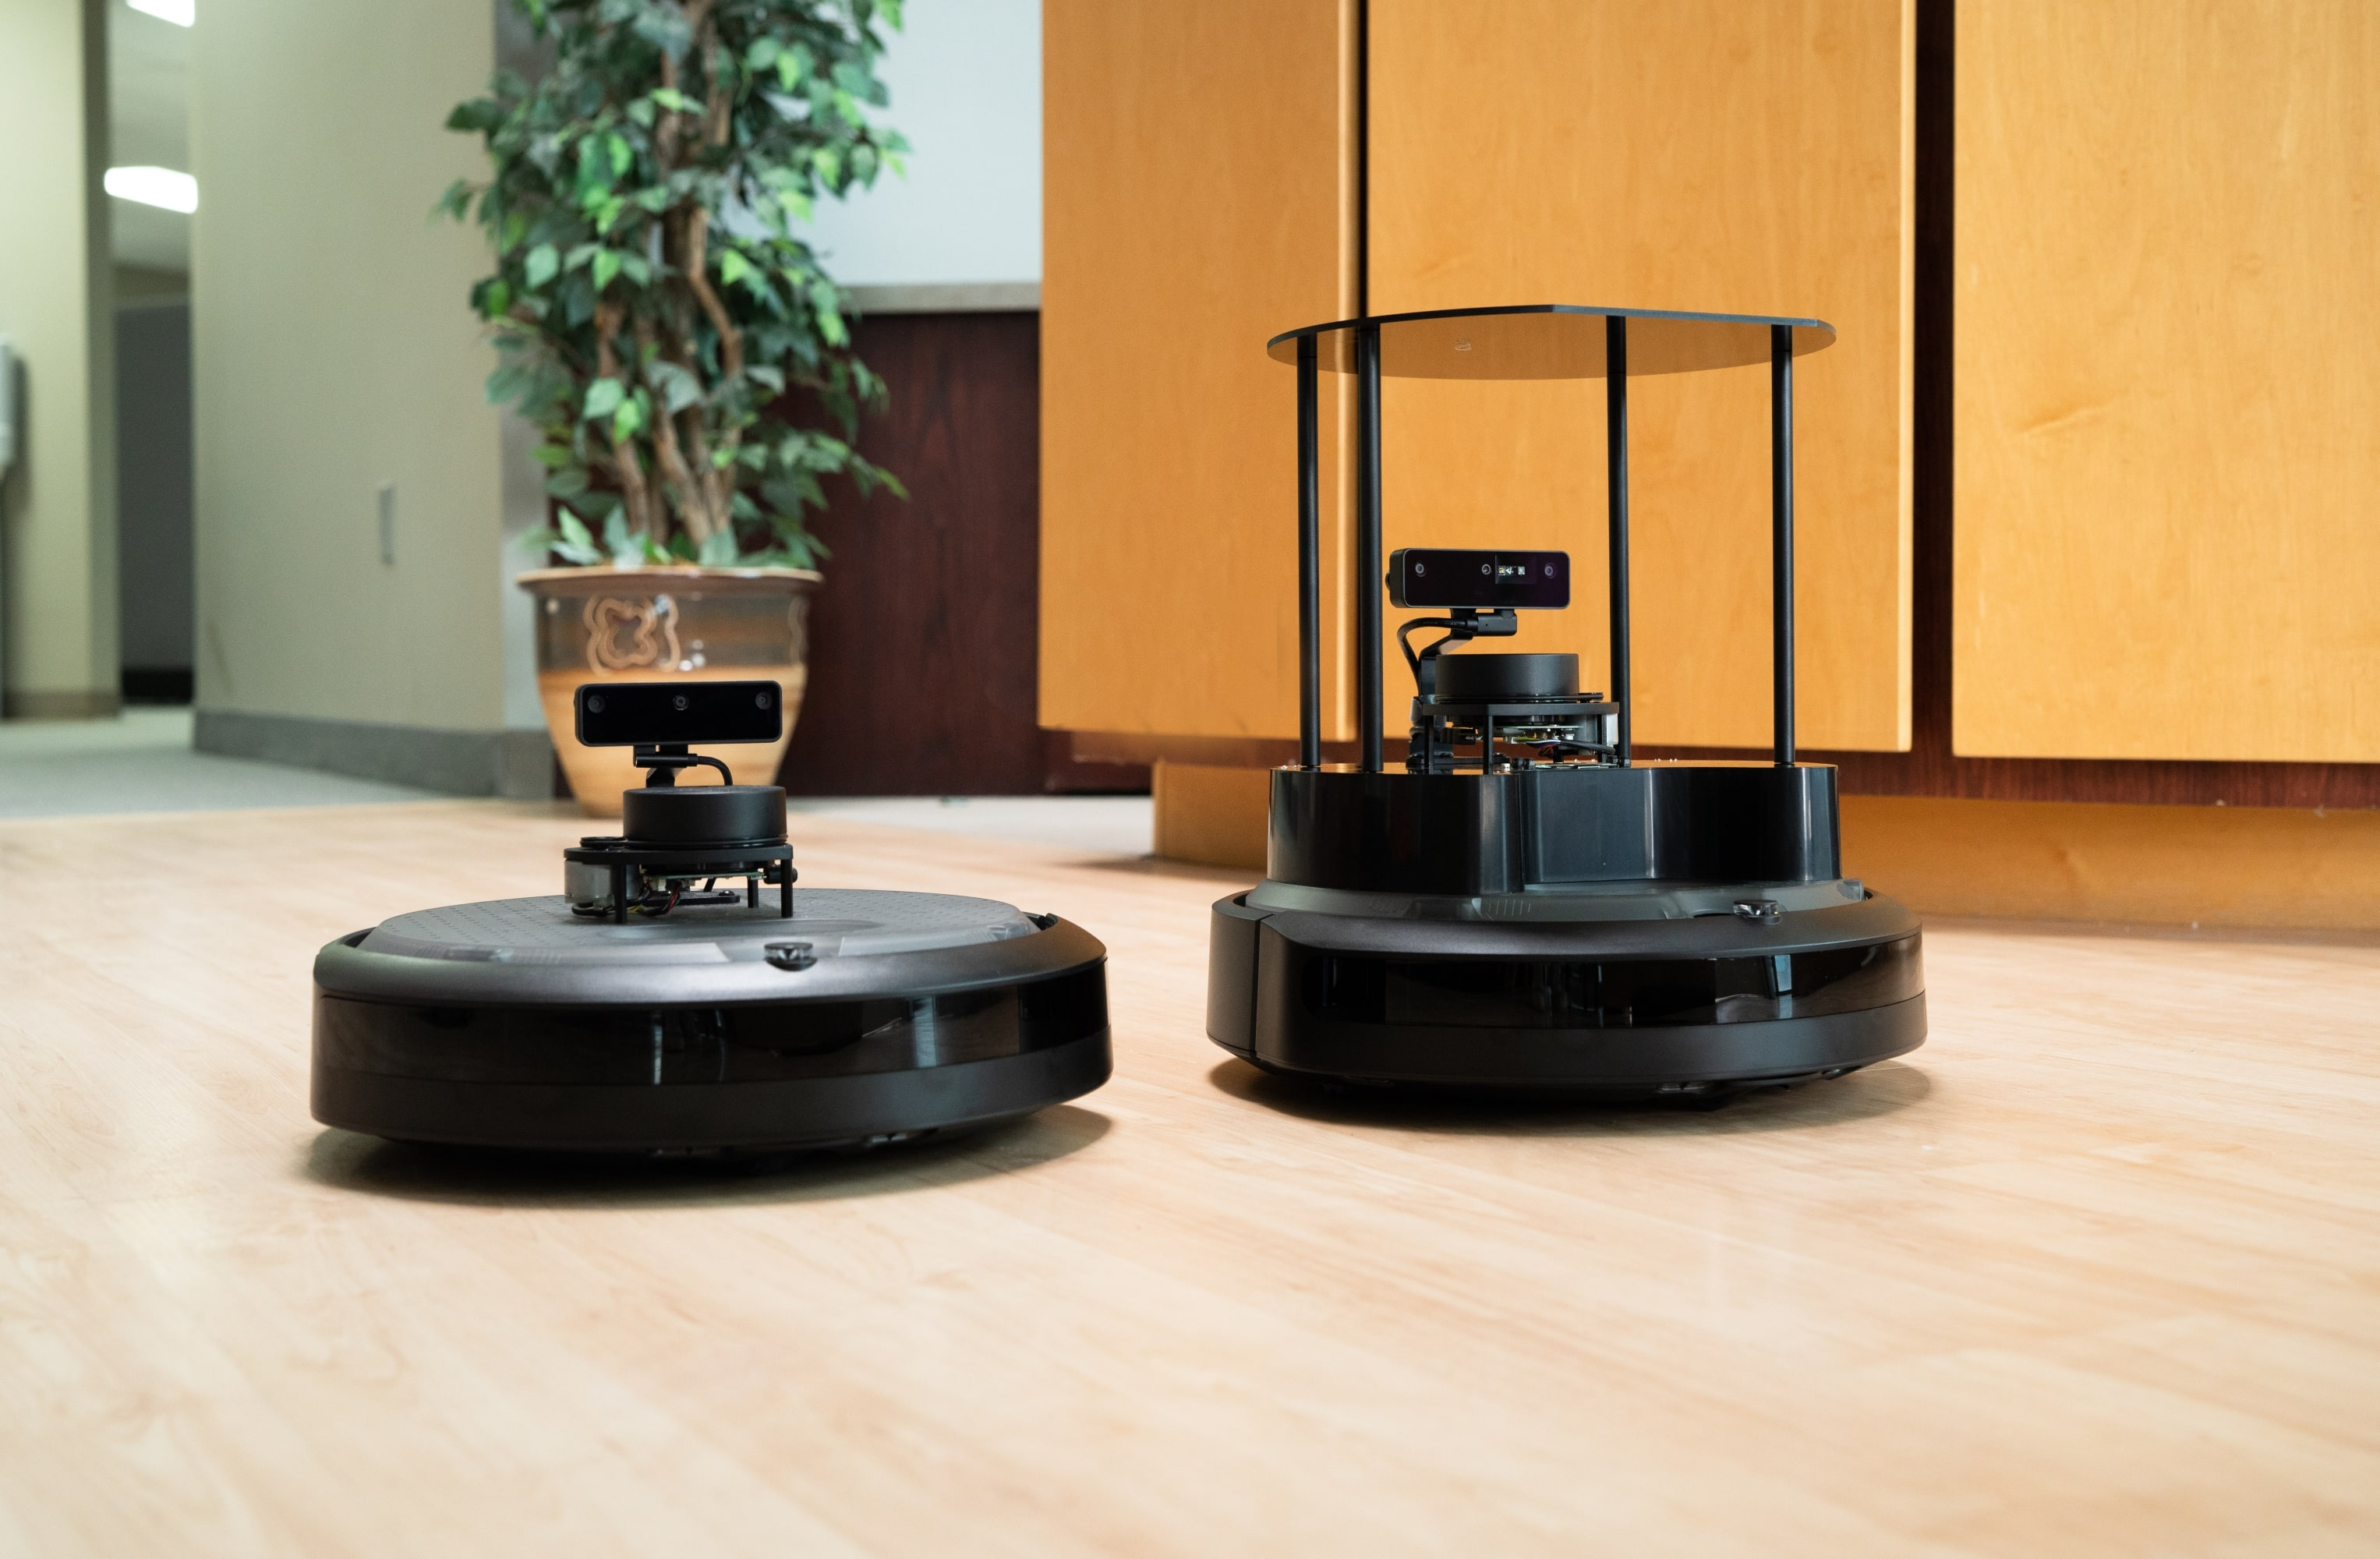
\includegraphics[width=0.62\textwidth]
    {images/chapter1/turtlebot4_lite.png}
    \caption{Nền tảng robot TurtleBot4 Lite sử dụng trong đề tài}
    \label{fig:turtlebot4-lite}

    \vspace{2pt}
    {\footnotesize\textit{Nguồn: TurtleBot 4 User Manual}}
\end{figure}


TurtleBot4 Lite hỗ trợ các thành phần cảm biến và thông tin trạng thái quan trọng:

\begin{itemize}
    \item LiDAR hai chiều phục vụ phát hiện vật cản và xây dựng bản đồ môi trường.
    \item Camera RGB hoặc camera RGB-D phục vụ quan sát và nhận diện đối tượng.
    \item Encoder bánh xe phục vụ ước lượng quãng đường và vận tốc chuyển động.
    \item IMU phục vụ đo vận tốc góc và hỗ trợ ước lượng trạng thái.
    \item Odometry biểu diễn vị trí và hướng tương đối của robot theo thời gian.
    \item Hệ thống TF quản lý quan hệ hình học giữa các hệ tọa độ của robot, cảm biến, bản đồ và mục tiêu.
\end{itemize}

Bên cạnh đó, TurtleBot4 được hỗ trợ bởi các công cụ phổ biến trong ROS2 như SLAM Toolbox, Nav2, RViz2 và Gazebo/Ignition. Điều này cho phép xây dựng một quy trình phát triển theo từng bước: kiểm thử thuật toán trong mô phỏng, đánh giá tính ổn định của hệ thống và chuẩn bị cho quá trình triển khai trên phần cứng thật.

Việc sử dụng môi trường mô phỏng Gazebo/Ignition giúp giảm chi phí thử nghiệm, hạn chế rủi ro va chạm cơ khí và tạo điều kiện quan sát trực quan dữ liệu cảm biến. Ngoài ra, mô phỏng cho phép thay đổi môi trường, vị trí vật cản và mục tiêu một cách linh hoạt mà không cần thiết lập lại không gian thử nghiệm thực tế.

\subsection{Bài toán nghiên cứu}

Bài toán đặt ra là xây dựng một hệ thống robot TurtleBot4 Lite có khả năng thực hiện nhiệm vụ tuần tra trong môi trường mô phỏng, phát hiện một đối tượng mục tiêu từ dữ liệu camera và chủ động di chuyển đến vị trí phù hợp gần đối tượng.

Trong quá trình hoạt động, robot cần thực hiện tuần tự các chức năng sau:

\begin{enumerate}
    \item Thu nhận dữ liệu từ LiDAR, camera, odometry và TF.
    
    \item Xây dựng hoặc sử dụng bản đồ môi trường đã được thiết lập trước.
    
    \item Xác định vị trí hiện tại của robot trên bản đồ.
    
    \item Di chuyển theo các điểm tuần tra được cấu hình trước.
    
    \item Nhận diện đối tượng mục tiêu từ ảnh RGB bằng mô hình YOLOv8n.
    
    \item Ước lượng vị trí tương đối của mục tiêu so với camera và robot.
    
    \item Chuyển đổi vị trí mục tiêu sang hệ tọa độ bản đồ thông qua TF.
    
    \item Tạo điểm đích phù hợp để robot tiếp cận mục tiêu mà không gây va chạm.
    
    \item Gửi điểm đích đến Nav2 và theo dõi trạng thái thực hiện nhiệm vụ.
    
    \item Sau khi hoàn thành nhiệm vụ tiếp cận, robot có thể quay lại chu trình tuần tra.
\end{enumerate}

Luồng xử lý tổng quát của hệ thống được mô tả như sau:

\begin{center}
\textit{Cảm biến $\rightarrow$ Xử lý dữ liệu $\rightarrow$ Định vị và lập bản đồ 
$\rightarrow$ Nhận diện mục tiêu $\rightarrow$ Lập kế hoạch đường đi 
$\rightarrow$ Điều khiển vận tốc $\rightarrow$ Cơ cấu chấp hành}
\end{center}

\subsection{Mục tiêu của đề tài}

Mục tiêu tổng quát của đề tài là xây dựng và phân tích một hệ thống robot tự hành TurtleBot4 Lite có khả năng tuần tra, nhận diện và tiếp cận mục tiêu trong môi trường mô phỏng.

Các mục tiêu cụ thể gồm:

\begin{itemize}
    \item Thiết lập môi trường mô phỏng TurtleBot4 Lite trên ROS2 Humble và Gazebo/Ignition.
    
    \item Khảo sát các nguồn dữ liệu cảm biến và thông tin trạng thái quan trọng như LiDAR, camera, encoder, odometry và TF.
    
    \item Sử dụng SLAM Toolbox để xây dựng bản đồ hai chiều của môi trường hoạt động.
    
    \item Sử dụng Nav2 để định vị, lập kế hoạch đường đi và điều hướng robot đến vị trí mong muốn.
    
    \item Tích hợp mô hình YOLOv8n để phát hiện đối tượng mục tiêu từ ảnh RGB.
    
    \item Ước lượng vị trí tương đối của mục tiêu từ dữ liệu ảnh và thông tin camera.
    
    \item Chuyển đổi tọa độ mục tiêu từ hệ tọa độ camera sang hệ tọa độ robot và hệ tọa độ bản đồ.
    
    \item Xây dựng Mission Manager để điều phối các trạng thái hoạt động như tuần tra, phát hiện mục tiêu, tiếp cận mục tiêu và quay lại nhiệm vụ ban đầu.
    
    \item Phân tích vai trò của cơ cấu chấp hành vi sai trong việc biến đổi lệnh vận tốc thành chuyển động thực tế của robot.
\end{itemize}

\subsection{Yêu cầu kỹ thuật của hệ thống}

Để hoàn thành nhiệm vụ, hệ thống cần đáp ứng các yêu cầu kỹ thuật cơ bản sau:

\begin{itemize}
    \item Robot có thể khởi chạy ổn định trong môi trường mô phỏng Gazebo/Ignition.
    
    \item Các topic cảm biến cần thiết được publish đúng định dạng và có thể quan sát trên RViz2.
    
    \item Dữ liệu LiDAR được sử dụng để xây dựng bản đồ và hỗ trợ tránh vật cản.
    
    \item Dữ liệu odometry và TF được cập nhật liên tục để xác định trạng thái chuyển động của robot.
    
    \item Nav2 có thể nhận goal pose, lập kế hoạch và phát lệnh vận tốc điều khiển robot.
    
    \item Mô hình nhận diện có thể phát hiện đối tượng mục tiêu từ luồng ảnh RGB.
    
    \item Khi sử dụng dữ liệu depth, hệ thống có thể ước lượng khoảng cách từ camera đến mục tiêu.
    
    \item Mission Manager có thể chuyển đổi hợp lý giữa các trạng thái hoạt động của robot.
    
    \item Các module được thiết kế tương đối độc lập để thuận tiện cho kiểm thử và mở rộng.
\end{itemize}

\subsection{Kiến trúc tổng quát của hệ thống}

Kiến trúc tổng quát của hệ thống được minh họa trong 
Hình~\ref{fig:system-architecture}. Hệ thống được tổ chức theo chuỗi xử lý 
khép kín: dữ liệu cảm biến được thu nhận và xử lý để xác định trạng thái 
của robot và môi trường; Mission Manager lựa chọn hành vi phù hợp; Nav2 
sinh lệnh vận tốc; cơ cấu truyền động vi sai tạo ra chuyển động thực tế 
và cung cấp thông tin phản hồi cho chu kỳ tiếp theo.

\begin{figure}[H]
    \centering

    \resizebox{0.98\textwidth}{!}{
    \begin{tikzpicture}[
        font=\small,
        node distance=0.75cm and 0.85cm,
        block/.style={
            rectangle,
            rounded corners=3pt,
            draw=black,
            thick,
            align=center,
            minimum height=1.0cm,
            minimum width=2.8cm,
            text width=2.8cm
        },
        sensor/.style={
            block,
            fill=blue!10
        },
        process/.style={
            block,
            fill=orange!15
        },
        manager/.style={
            block,
            fill=green!15,
            minimum width=3.3cm,
            text width=3.3cm
        },
        actuator/.style={
            block,
            fill=red!10
        },
        arrow/.style={
            -{Stealth[length=2.5mm]},
            thick
        }
    ]

    % ================= LỚP CẢM BIẾN =================
    \node[sensor] (lidar)
        {LiDAR\\Quét môi trường};

    \node[sensor, right=of lidar] (camera)
        {Camera RGB-D\\Ảnh màu và depth};

    \node[sensor, right=of camera] (encoder)
        {Encoder và IMU\\Thông tin trạng thái};

    % ================= LỚP XỬ LÝ =================
    \node[process, below=of lidar] (slam)
        {SLAM Toolbox\\Bản đồ và pose};

    \node[process, below=of camera] (vision)
        {YOLOv8n\\Nhận diện mục tiêu};

    \node[process, below=of encoder] (tf)
        {Odometry và TF\\Biến đổi tọa độ};

    % ================= QUẢN LÝ NHIỆM VỤ =================
    \node[manager, below=1.05cm of vision] (mission)
        {Mission Manager\\Tuần tra và tiếp cận mục tiêu};

    % ================= ĐIỀU KHIỂN VÀ CHẤP HÀNH =================
    \node[process, below left=0.95cm and -0.15cm of mission] (nav2)
        {Nav2\\Lập kế hoạch và điều hướng};

    \node[actuator, below right=0.95cm and -0.15cm of mission] (drive)
        {Cơ cấu chấp hành\\Truyền động vi sai};

    % ================= MŨI TÊN =================
    \draw[arrow] (lidar) -- (slam);
    \draw[arrow] (camera) -- (vision);
    \draw[arrow] (encoder) -- (tf);

    \draw[arrow] (slam) -- (mission);
    \draw[arrow] (vision) -- (mission);
    \draw[arrow] (tf) -- (mission);

    \draw[arrow] (mission) -- (nav2);
    \draw[arrow] (nav2) --
        node[above, sloped] {\texttt{/cmd\_vel}}
        (drive);

    \draw[arrow, dashed] (drive.east)
        to[out=0, in=0, looseness=1.65]
        node[right, align=left] {Phản hồi\\trạng thái}
        (encoder.east);

    \end{tikzpicture}
    }

    \caption{Kiến trúc tổng quát của hệ thống robot tự hành TurtleBot4 Lite}
    \label{fig:system-architecture}
\end{figure}

Hệ thống được chia thành các nhóm module chính như sau:


\begin{enumerate}
    \item \textbf{Module mô phỏng và bringup:}
    
    Khởi tạo robot TurtleBot4 Lite, môi trường Gazebo/Ignition, mô hình URDF và các node ROS2 cần thiết.
    
    \item \textbf{Module cảm biến và thông tin trạng thái:}
    
    Thu nhận dữ liệu LiDAR, camera, odometry và TF. Module này đóng vai trò cung cấp dữ liệu đầu vào cho các khối xử lý phía sau.
    
    \item \textbf{Module SLAM và localization:}
    
    Xây dựng bản đồ môi trường hoặc xác định pose hiện tại của robot trên bản đồ đã có.
    
    \item \textbf{Module navigation:}
    
    Sử dụng Nav2 để lập kế hoạch đường đi, tránh vật cản và sinh lệnh vận tốc tuyến tính, vận tốc góc cho robot.
    
    \item \textbf{Module perception:}
    
    Sử dụng mô hình YOLOv8n để nhận diện đối tượng mục tiêu từ ảnh RGB. Khi có dữ liệu depth, module thực hiện bổ sung bước ước lượng vị trí tương đối của mục tiêu.
    
    \item \textbf{Module Mission Manager:}
    
    Quản lý trạng thái hoạt động của hệ thống, điều phối quá trình tuần tra, tạm dừng, tiếp cận mục tiêu và tiếp tục nhiệm vụ.
\end{enumerate}

\subsection{Phạm vi nghiên cứu}

Đề tài tập trung vào việc mô phỏng và tích hợp các thành phần cơ bản của một hệ robot tự hành. Robot sử dụng là TurtleBot4 Lite hoạt động trong môi trường warehouse của Gazebo/Ignition. Phần mềm được triển khai trên ROS2 Humble.

Môi trường mô phỏng TurtleBot4 Lite trong Ignition Gazebo được minh họa 
trong Hình~\ref{fig:turtlebot4-ignition-gazebo}. Việc sử dụng mô phỏng 
cho phép kiểm tra hoạt động của robot, luồng dữ liệu cảm biến và thuật toán 
điều hướng trước khi triển khai trên phần cứng thật.

\begin{figure}[H]
    \centering
    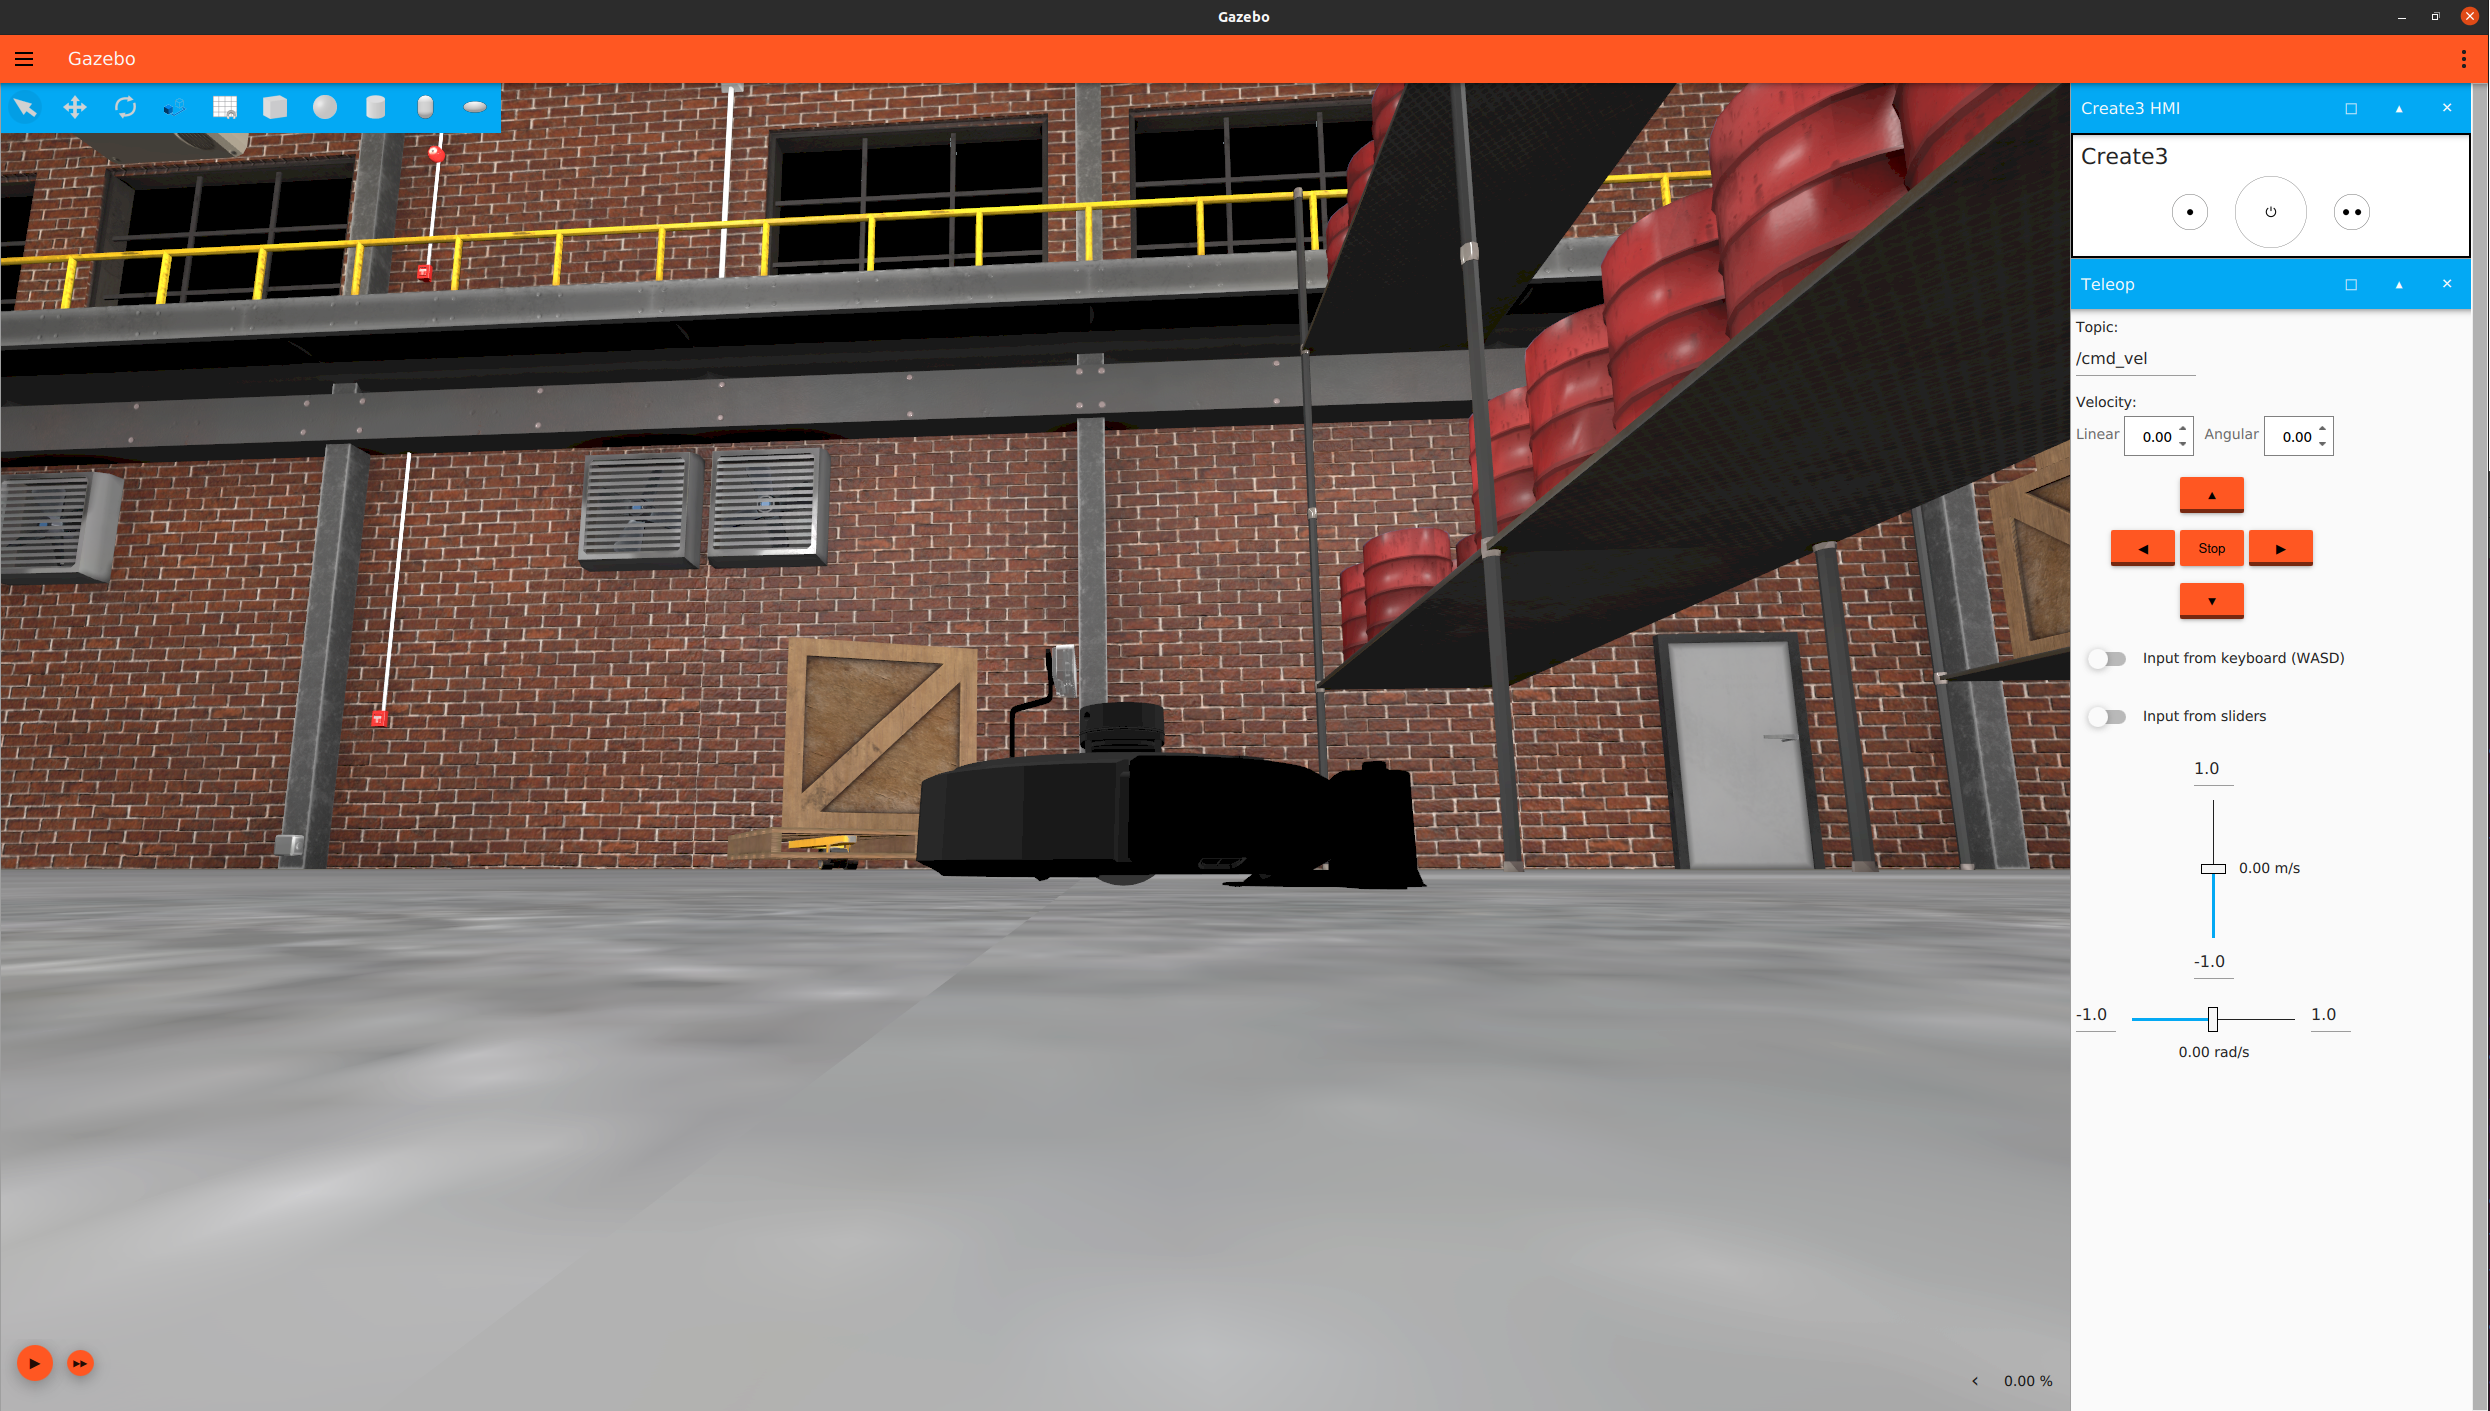
\includegraphics[width=0.88\textwidth]
    {images/chapter1/turtlebot4_gazebo.png}
    \caption{TurtleBot4 Lite trong môi trường mô phỏng Ignition Gazebo}
    \label{fig:turtlebot4-ignition-gazebo}

    \vspace{2pt}
    {\footnotesize\textit{Nguồn: TurtleBot 4 User Manual}}
\end{figure}

Trong phạm vi báo cáo, hệ thống tập trung vào các nội dung sau:

\begin{itemize}
    \item Khởi tạo robot và môi trường mô phỏng.
    
    \item Quan sát và phân tích dữ liệu LiDAR, camera, odometry và TF.
    
    \item Lập bản đồ hai chiều bằng SLAM Toolbox.
    
    \item Điều hướng robot bằng Nav2.
    
    \item Nhận diện đối tượng mục tiêu bằng YOLOv8n pretrained trên tập dữ liệu COCO.
    
    \item Xây dựng logic quản lý nhiệm vụ cơ bản.
\end{itemize}

Một số nội dung chưa được triển khai chuyên sâu trong phạm vi đề tài gồm:

\begin{itemize}
    \item Tối ưu hóa tham số Nav2 cho từng loại môi trường cụ thể.
    
    \item Theo dõi đồng thời nhiều đối tượng chuyển động.
    
    \item Xử lý tình huống mục tiêu bị che khuất hoặc mất khỏi trường nhìn camera.
    
    \item Huấn luyện lại mô hình nhận diện trên tập dữ liệu chuyên biệt.
    
    \item Tối ưu hiệu năng xử lý ảnh trên phần cứng nhúng.
    
    \item Đánh giá đầy đủ độ chính xác khi triển khai trên robot TurtleBot4 thật.
\end{itemize}

\subsection{Phương pháp thực hiện}

Quy trình thực hiện đề tài được chia thành các giai đoạn:

\begin{enumerate}
    \item Nghiên cứu cấu trúc phần cứng và phần mềm của TurtleBot4 Lite.
    
    \item Thiết lập ROS2 Humble và môi trường mô phỏng Gazebo/Ignition.
    
    \item Kiểm tra các topic, frame và node liên quan đến cảm biến, cơ cấu chấp hành và trạng thái robot.
    
    \item Chạy thử SLAM Toolbox để xây dựng bản đồ môi trường.
    
    \item Chạy thử Nav2 để điều hướng robot đến các goal pose định trước.
    
    \item Tích hợp mô hình YOLOv8n để nhận diện đối tượng từ camera.
    
    \item Xây dựng module ước lượng vị trí và module quản lý nhiệm vụ.
    
    \item Đánh giá kết quả, phân tích hạn chế và đề xuất hướng phát triển.
\end{enumerate}

\subsection{Đóng góp chính của báo cáo}

Báo cáo không chỉ trình bày quy trình khởi chạy một hệ thống ROS2 mà còn phân tích vai trò kỹ thuật của từng thành phần dưới góc nhìn cảm biến và cơ cấu chấp hành.

Các đóng góp chính gồm:

\begin{itemize}
    \item Đề xuất kiến trúc module cho hệ robot TurtleBot4 Lite thực hiện nhiệm vụ tuần tra và tiếp cận mục tiêu.
    
    \item Phân tích vai trò của LiDAR, camera, encoder, odometry và TF trong hệ robot tự hành.
    
    \item Trình bày chuỗi xử lý dữ liệu từ cảm biến đến bản đồ, pose robot và vị trí mục tiêu.
    
    \item Phân tích cơ cấu truyền động vi sai và quá trình Nav2 sinh lệnh vận tốc điều khiển robot.
    
    \item Xây dựng luồng nhiệm vụ kết hợp patrol, perception, localization và navigation.
    
    \item Đánh giá các kết quả đạt được, những hạn chế còn tồn tại và khả năng triển khai trên robot thật.
\end{itemize}

\subsection{Kết quả kỳ vọng}

Sau khi hoàn thành đề tài, hệ thống kỳ vọng đạt được các kết quả sau:

\begin{itemize}
    \item Robot có thể hoạt động ổn định trong môi trường mô phỏng.
    
    \item Các dữ liệu cảm biến và thông tin trạng thái được hiển thị trực quan trên RViz2.
    
    \item Robot có thể xây dựng bản đồ môi trường và xác định vị trí tương đối trên bản đồ.
    
    \item Robot có thể nhận goal pose và tự động di chuyển đến vị trí được chỉ định.
    
    \item Hệ thống nhận diện có thể phát hiện đối tượng mục tiêu trong ảnh RGB.
    
    \item Mission Manager có thể điều phối luồng nhiệm vụ cơ bản từ tuần tra đến tiếp cận mục tiêu.
\end{itemize}

